\section{流映射}
\label{sec:transp-flow}

上一节一次只跟踪一条特征线。把所有特征线放在一起看，固定两个时刻，每个粒子从前一时刻的位置走到后一时刻的位置，这就是一个空间到自身的映射。第~\ref{chap:ode-sensitivity}章已经研究过它，这里把要用的结论写下来。

\paragraph{流映射回顾}
对速度场$\bm{v}$，流映射$\bm{\varphi}_{s,t}(\bm{x})$表示时刻$s$位于$\bm{x}$的粒子在时刻$t$的位置，即
\begin{equation}
  \partial_t\bm{\varphi}_{s,t}(\bm{x})=\bm{v}\bigl(\bm{\varphi}_{s,t}(\bm{x}),t\bigr),\qquad
  \bm{\varphi}_{s,s}(\bm{x})=\bm{x}.
  \label{eq:transp-flow}
\end{equation}
上一节的$\bm{X}(s;\bm{x},t)$就是$\bm{\varphi}_{t,s}(\bm{x})$。

在条件（V）下，$\bm{\varphi}_{s,t}$是$\mathbb{R}^{d}$到自身的$C^{1}$双射。第~\ref{chap:ode-sensitivity}章还给出了两条代数规则：走两段等于走一段，走过去再走回来回到原处，即
\begin{equation}
  \bm{\varphi}_{r,t}\circ\bm{\varphi}_{s,r}=\bm{\varphi}_{s,t},\qquad
  \bm{\varphi}_{t,s}=\bm{\varphi}_{s,t}^{-1}.
  \label{eq:transp-flow-rules}
\end{equation}

\paragraph{输运解的表示}
用流映射重写式~\eqref{eq:transp-char-solution}，得到
\begin{equation}
  u(\cdot,t)=u_0\circ\bm{\varphi}_{t,0}+\int_0^{t}f(\cdot,s)\circ\bm{\varphi}_{t,s}\,\mathrm{d}s.
  \label{eq:transp-flow-solution}
\end{equation}
这里出现的是逆向的映射$\bm{\varphi}_{t,0}$。粒子带着值$u_0(\bm{x}_0)$从$\bm{x}_0$走到$\bm{\varphi}_{0,t}(\bm{x}_0)$，要想知道固定位置$\bm{y}$的值，必须先问“现在位于$\bm{y}$的粒子原来在哪里”，然后到初值里去查。

图~\ref{fig:transp-lookup}把例~\ref{ex:transp-stretch}的三个粒子连了起来。这时$\varphi_{0,\ln2}(x)=2x$，上下两条曲线上用箭头相连的点高度相同。要读下面的曲线在$y=3$处的值，就从$y=3$沿箭头退回$x_0=1.5$，到上面的曲线上读出$0.5$。

\begin{BookInlineFigure}
  \centering
  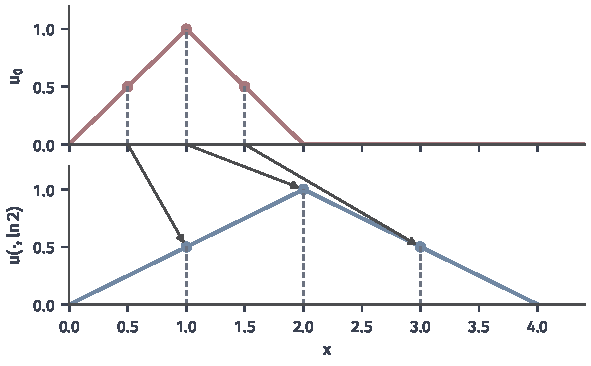
\includegraphics[width=100mm]{figures/06-differential-equations/02-partial-differential-equations/matplotlib/transp-lookup/figure.pdf}
  \caption{用流映射搬运场值，$v=x$，$t=\ln2$。上图是初值（红），下图是搬运后的解（蓝）。箭头把位置$x_0=0.5,1,1.5$连到$2x_0$，点的高度保持不变。}
  \label{fig:transp-lookup}
\end{BookInlineFigure}

同一个解有两种描述方式。跟着粒子看，$u(\bm{\varphi}_{0,t}(\bm{x}_0),t)=u_0(\bm{x}_0)$，这称为\term{Lagrange描述}（Lagrangian description），标号是粒子的初始位置。站在固定位置看，$u(\bm{y},t)=u_0(\bm{\varphi}_{t,0}(\bm{y}))$，这称为\term{Euler描述}（Eulerian description），标号是当前位置。两者用流映射互相转换，这也是公式中需要逆映射的原因。

$v=x$时流映射是$\varphi_{s,t}(x)=x\mathrm{e}^{t-s}$。规则~\eqref{eq:transp-flow-rules}在这里就是指数的相加。$v=xt$时流映射依赖两个时刻：
\[
  \varphi_{s,t}(x)=x\exp\Bigl(\frac{t^{2}-s^{2}}{2}\Bigr).
\]
这时$\varphi_{0,1}$的倍数是$\mathrm{e}^{1/2}$，$\varphi_{1,2}$的倍数是$\mathrm{e}^{3/2}$，相乘得到$\varphi_{0,2}$的倍数$\mathrm{e}^{2}$，符合式~\eqref{eq:transp-flow-rules}；但第二段时间的倍数不等于第一段，同样长的时间间隔走出的倍数不同，所以必须记住起止两个时刻。

平面上的情形类似。旋转场$\bm{v}=(-x_2,x_1)^{\top}$的流映射是旋转矩阵，鞍点场$\bm{v}=(x_1,-x_2)^{\top}$沿一个方向拉伸，沿另一个方向压缩：
\[
  \bm{\varphi}_{t}^{\mathrm{rot}}(\bm{x})=
  \begin{pmatrix}\cos t&-\sin t\\ \sin t&\cos t\end{pmatrix}\bm{x},\qquad
  \bm{\varphi}_{t}^{\mathrm{sad}}(\bm{x})=
  \begin{pmatrix}\mathrm{e}^{t}&0\\ 0&\mathrm{e}^{-t}\end{pmatrix}\bm{x}.
\]

图~\ref{fig:transp-2d-advect}用式~\eqref{eq:transp-flow-solution}搬运了一个由两团组成的初值。旋转把它转了四分之一圈，形状不变；鞍点流把它在一个方向拉长、另一个方向压扁。两种情形下，解的最大值都和初值相同，因为$u$只是被搬动，没有哪个粒子携带的值发生了变化。

\begin{BookInlineFigure}
  \centering
  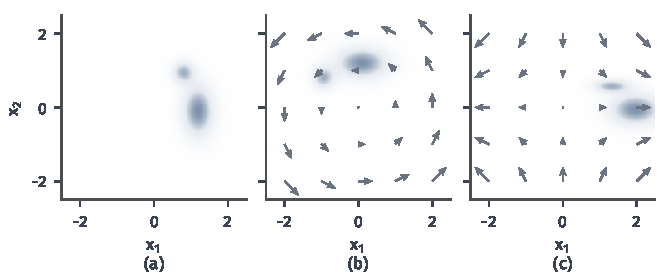
\includegraphics[width=112mm]{figures/06-differential-equations/02-partial-differential-equations/matplotlib/transp-2d-advect/figure.pdf}
  \caption{平面上的搬运，蓝色越深值越大，三幅图共用一个色阶，灰色箭头是速度场的方向。(a)初值。(b)旋转场，$t=\pi/2$。(c)鞍点场$\bm{v}=(x_1,-x_2)^{\top}$，$t=0.5$。}
  \label{fig:transp-2d-advect}
\end{BookInlineFigure}

\paragraph{逆映射的范围}
条件（V）保证了粒子不会在有限时间内跑到无穷远，也就保证了$\bm{\varphi}_{s,t}$在全空间上定义。去掉全局Lipschitz条件后，轨迹可能爆炸，逆映射的定义域就受到限制。

取$v=x^{2}$，第~\ref{chap:ode-sensitivity}章已经算出它的流映射：
\[
  \varphi_{0,t}(x)=\frac{x}{1-tx},\qquad x<\frac1t\quad(t>0).
\]
当$x$跑遍$(-\infty,1/t)$时，$\varphi_{0,t}(x)$跑遍$(-1/t,\infty)$。于是从初始线出发的粒子在时刻$t$只占据$y>-1/t$，反解得到的逆映射只在这个范围内有定义：
\[
  \varphi_{t,0}(y)=\frac{y}{1+ty},\qquad y>-\frac1t.
\]

图~\ref{fig:transp-flow-domain}(a)中，浅红色区域$\{x\leq-1/t\}$里的点没有来自初始线的特征线，它们的值由初值无法确定，这些特征线要追溯到“从$-\infty$进来”。另一方面，$x_0\geq1/t$的粒子在时刻$t$之前已经跑到了$+\infty$。例如$(y,t)=(1,1)$的出发位置是$1/2$，而$(y,t)=(-2,1)$没有出发位置。

\begin{BookInlineFigure}
  \centering
  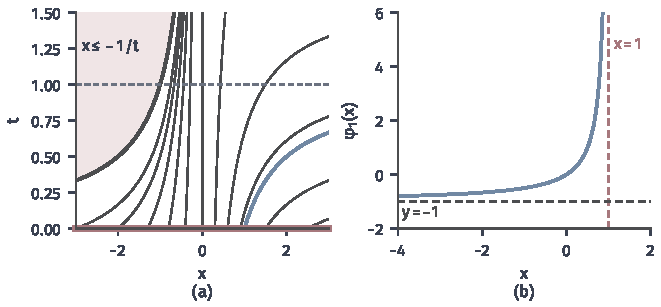
\includegraphics[width=112mm]{figures/06-differential-equations/02-partial-differential-equations/matplotlib/transp-flow-domain/figure.pdf}
  \caption{速度场$v=x^{2}$的流映射只在部分区域可逆。(a)特征线（深灰），蓝线是从$x_0=1$出发、在$t=1$爆炸的轨迹，粗深灰线$x=-1/t$是从初始线可达区域的边界，浅红区域无法追溯到初始线。(b)$\varphi_{0,1}(x)=x/(1-x)$，定义在$x<1$，值域是$(-1,\infty)$。}
  \label{fig:transp-flow-domain}
\end{BookInlineFigure}

所以一般情形下，式~\eqref{eq:transp-flow-solution}只在点$(\bm{y},t)$的反向轨迹能够回到$t=0$时才有意义。这时解存在的区域是流映射的值域，而不是整个时空。

\paragraph{轨迹唯一性}
即使轨迹全局存在，失去唯一性也会破坏这种表示。取$v(x)=2\sqrt{\lvert x\rvert}$，它在$x=0$处不Lipschitz。从负轴出发的粒子向右运动，在有限时间到达$0$，然后可以在$0$停留任意一段时间，再离开。过$(0,c)$向右离开的轨迹是$x=(t-c)^{2}$。

看图~\ref{fig:transp-nonunique}(a)中的点$P=(1,2)$。反向追踪得到$x=(r-1)^{2}$，在$r=1$到达$0$。再往回，有多条轨迹都能走到$(0,1)$：可以一直停在$0$，也可以来自负轴。凡是出发位置$x_0\in[-1,0]$的粒子，都可能在时刻$2$到达$P$，图中用红色粗线标出这些出发位置，黄色虚线是其中两条。

如果$u$是$C^{1}$解，它沿每条这样的轨迹都不变，所以$u_0$在$[-1,0]$上必须是常数。只要初值在这一段上不是常数，方程就没有$C^{1}$解。

\begin{BookInlineFigure}
  \centering
  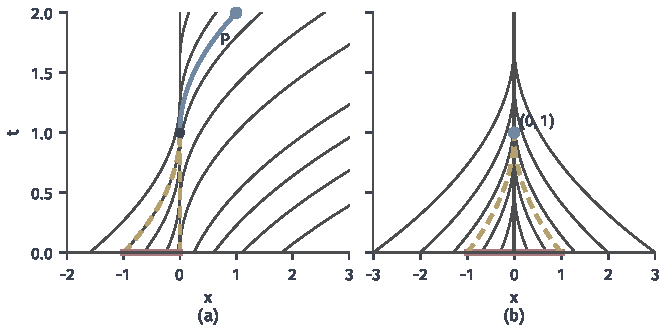
\includegraphics[width=112mm]{figures/06-differential-equations/02-partial-differential-equations/matplotlib/transp-nonunique/figure.pdf}
  \caption{速度场不Lipschitz时的轨迹。(a)$v=2\sqrt{\lvert x\rvert}$，轨迹在$x=0$处分叉，蓝线是到达$P$的最后一段，黄色虚线是到达$(0,1)$的两条路径，红色粗线是可能的出发位置$[-1,0]$。(b)$v=-2\,\mathrm{sgn}(x)\sqrt{\lvert x\rvert}$，轨迹并入$x=0$，从蓝点反向追踪的出发位置是红色粗线$[-1,1]$。}
  \label{fig:transp-nonunique}
\end{BookInlineFigure}

图~\ref{fig:transp-nonunique}(b)是反方向的情形。$v=-2\,\mathrm{sgn}(x)\sqrt{\lvert x\rvert}$下，粒子都流向$0$，正向轨迹是唯一的，但$[-1,1]$中的粒子在$t=1$时都已并入$0$，$\varphi_{0,1}$不是单射，逆映射不存在。从$(0,1)$反向追踪得到一整段出发位置，$u_0$在$[-1,1]$上不是常数时，同样不存在$C^{1}$解。

这两个例子说明，输运解的表示依赖于$\bm{\varphi}_{s,t}$的可逆性，可逆性又依赖轨迹在正反两个方向上的唯一性。以下都假设条件（V），需要讨论局部情形时，会明确说明定义域。
